%!TEX root = ../thesis.tex

本章では，提案手法のシステム構成について述べる．\Fig{fig:system} に示すように，本手法は，(1) 物体検出，(2) 物体追跡，(3) セグメンテーション，の3つのモジュールで構成される．以下にそれぞれのモジュールに関して述べる．

\begin{figure}[H]
\centering
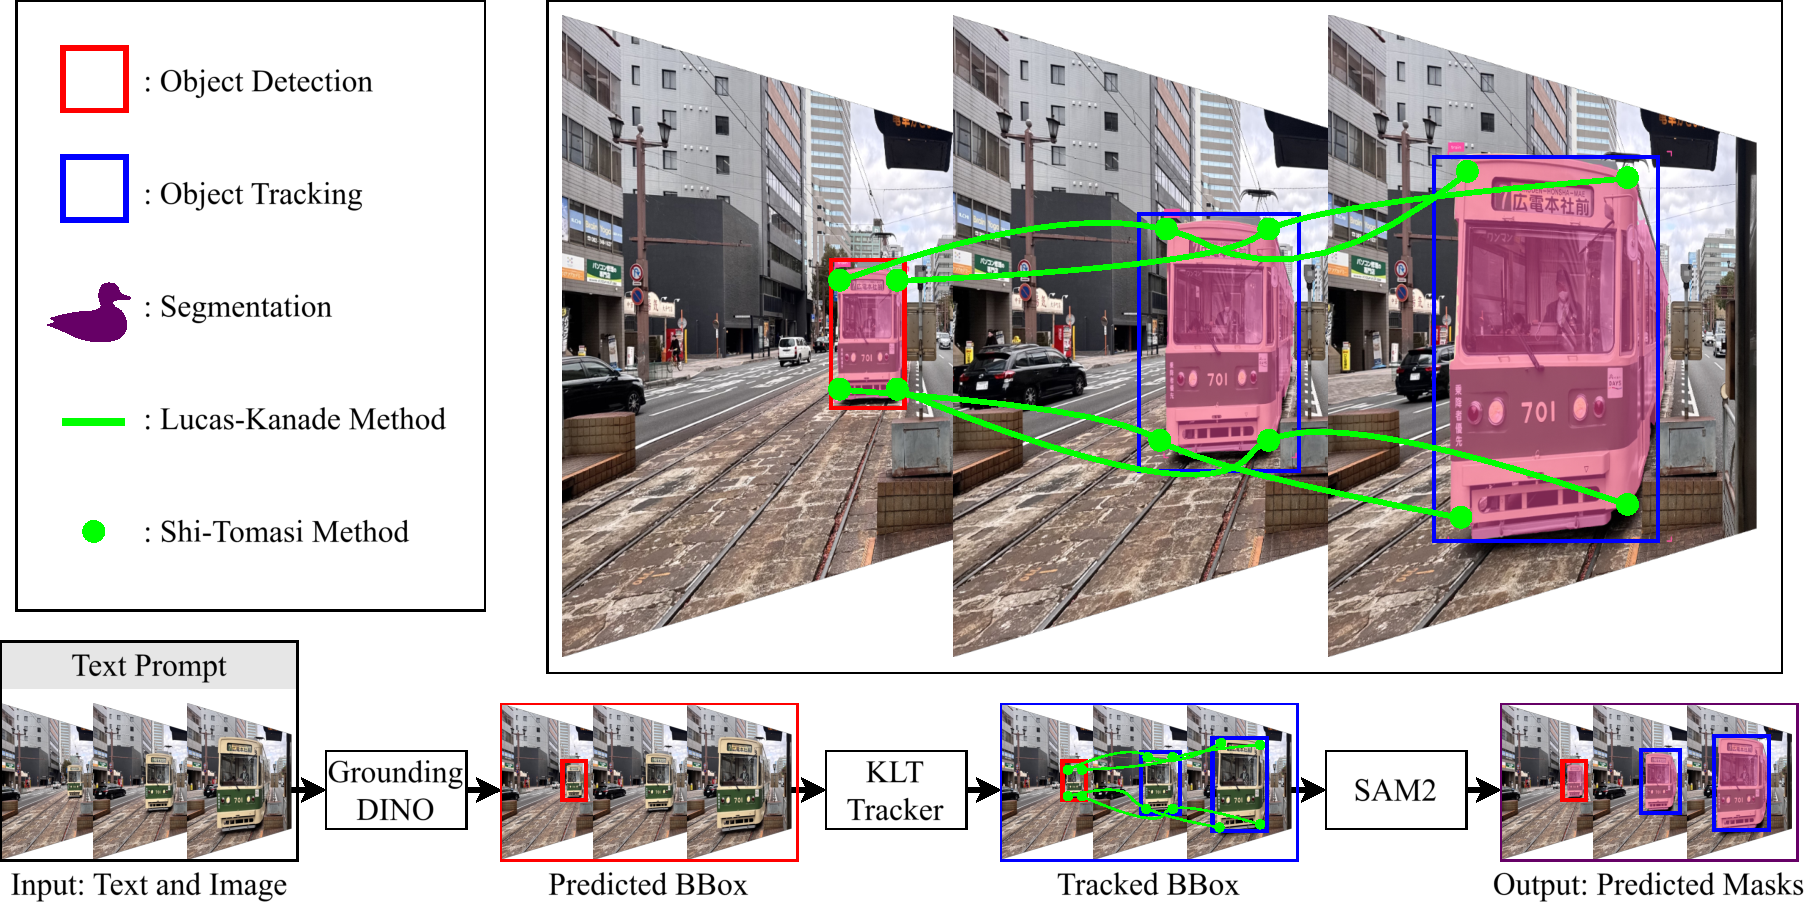
\includegraphics[width=1.0\linewidth]{images/pdf/system_ver1.pdf}
\caption{Overview of the system.}
\label{fig:system}
\end{figure}

\newpage

\section{物体検出モジュール}
テキストプロンプトに基づき，Grounding DINOを用いて物体検出を行う．これによって，テキストに対応するバウンディングボックスが生成される．この処理は，毎フレームではなく一定間隔で実行し，計算負荷が過大とならないようにする．

\section{物体追跡モジュール}
後続のフレームでは，毎フレームGrounding DINOを実行する代わりに，物体追跡でBBoxを更新する．まず，前フレームのBBox内でShi-Tomasi法 \cite{shi_tomasi} に基づき画像特徴点を抽出する．次に，抽出した特徴点群をLucas-Kanade法 \cite{lucas_kanade} に基づくピラミッドオプティカルフローで追跡し，その移動ベクトルの中央値を算出する．このベクトルを用いてBBoxの位置と大きさを更新する．以上の一連の処理を繰り返し実行する．これらの手法は，標準的かつ計算効率に優れていることから，特徴点追跡に採用した．

\section{セグメンテーションモジュール}
検出または追跡によって更新されたBBoxに対し，SAM2を用いてセグメンテーションマスクを生成する．これは，比較的小さいモデルを使用して毎フレーム実行する．これにより，検出から追跡，セグメンテーションまでの一連の処理を行う．

\newpage
